\documentclass{beamer}
\usepackage[spanish]{babel}
\usepackage[utf8]{inputenc}
\usepackage{tikz}
\usepackage[T1]{fontenc} 
\usepackage{calligra} 
\usetikzlibrary{arrows,automata}



% coding: utf-8

\newcommand{\ToDo}{\color{red} {\Huge COMPLETAR} \normalcolor}
\newcommand{\ReView}{\color{red} {\Huge REVISAR!! } \normalcolor}
\newcommand{\Ask}{\color{red} {\Huge CONSULTAR!! } \normalcolor}

\newcommand{\saltosinsangria}{ \newline \newline}


\newcommand{\filaparS}[2]
{
	{#1} & {#2}\\ 
}

\newcommand{\filaimparS}[2]
{
	{#1} & {#2}\\ 
}

\newcommand{\camposcolorS}[2]
{
\textbf{{#1}} & \textbf{{#2}}\\
}



\newcommand{\filaparT}[4]
{
	\rowcolor[gray]{1}{#1} & {#2} & {#3} & {#4}\\ 
}

\newcommand{\filaimparT}[4]
{
	\rowcolor[gray]{0.8}{#1} & {#2} & {#3} & {#4}\\ 
}

\newcommand{\camposcolorT}[4]
{
	\rowcolor[cmyk]{1,1,0,0} \textbf{\color{white} {#1}} & \textbf{\color{white} {#2}} & \textbf{\color{white} {#3}} & \textbf{\color{white} {#4}} \\
}

\newcommand{\filapar}[6]
{
	\rowcolor[gray]{1}{#1} & {#2} & {#3} & {#4} & {#5} & {#6}\\ 
}

\newcommand{\filaimpar}[6]
{
	\rowcolor[gray]{0.8}{#1} & {#2} & {#3} & {#4} & {#5} & {#6}\\ 
}

\newcommand{\camposcolor}[6]
{
	\rowcolor[cmyk]{1,1,0,0} \textbf{\color{white} {#1}} & \textbf{\color{white} {#2}} & \textbf{\color{white} {#3}} & \textbf{\color{white} {#4}} & \textbf{\color{white} {#5}} & \textbf{\color{white} {#6}}\\
}

\newcommand{\imagen}[3]
{
	\begin{figure}[p!hbt]
	  \centering
	  \includegraphics[scale=#3]{#1}
	  \caption{#2}
          \label{fig_#1}
	\end{figure}
} 

\newcommand{\imagenst}[2]
{
	\begin{figure}[p!hbt]
	  \centering
	  \includegraphics[scale=#2]{#1}
	\end{figure}
} 
\newcommand{\imagenvertical}[3]
{
	\begin{figure}[p!hbt]
	  \centering
	  \includegraphics[angle=90,scale=#3]{../img/#1}
	  \caption{#2}
          \label{fig_#1}
	\end{figure}
}

%\usetheme{Berkeley}
% \usetheme{JuanLesPins}
% \usetheme{bars}
% \usetheme{split}
  \usetheme[compress]{Ilmenau}
% \mode<presentation>
%\mode<handout>%{\beamertemplatesolidbackgroundcolor{black!5}}
% \mode<article>{\usepackage{fullpage}}
% \usepackage{pgfpages}
%\pgfpagelayout{resize}[a4paper,border shrink=5mm,landscape]

\include{epsfig}
\title{Matrices  definidas positivas}

\author{Christian Sebasti\'an Russo}
\date{16 de Septiembre de 2015}

\begin{document}

\frame{\titlepage}

\frame{\tableofcontents}

\section{Contexto}
\subsection{?`De d\'onde venimos?}

\frame{
\frametitle{?`De d\'onde venimos?} 
\begin{itemize}
\item Operaciones con matrices (suma, resta, permutaciones, etc.)
\item Eliminaci\'on Gaussiana
\item Factorizaci\'on LU
\item Te\'orica de Matrices definidas positivas
\item Te\'orica de Factorizaci\'on de Cholesky
\end{itemize}
}




\subsection{?`A d\'onde vamos?}

\frame{
\frametitle{Objetivos} 
\begin{itemize}
\item Dudas comunes
\item Primeros ejercicios Matrices definidas positivas
\item Ponernos cancheros con los ejercicios
\end{itemize}
}







\section{Matrices definidas positivas}
\subsection{Repaso}

\frame{
\frametitle{Repaso }

\textbf{Matriz Triangular Superior e Inferior:} 

\begin{center}
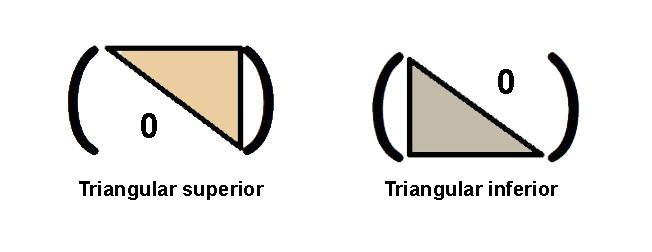
\includegraphics[width=0.5\textwidth]{triangulares.jpg}
\end{center}

\textbf{Proposici\'on:} Sea A una matriz triangular \[ det(L) = \prod_{i = 1}^n l_{ii}  \]
\textbf{Propiedad:} 
Sea v $\in$ $\mathbb{R}^{nx1}$. Entonces $v^t \cdot v = $ $\left\| v \right\| ^2$

\textbf{Propiedad:} 
Sea A una matriz inversible. Entonces la ecuaci\'on $Ax = 0$ tiene como \'unica soluci\'on x = 0
}


\subsection{Conceptos}

\frame{

\begin{center}

\includegraphics[width=1\textwidth]{isabelfinal.jpg}
\end{center}
\frametitle{Matrices definidas positivas}
\begin{block}{Definici\'on }
Sea A $\in$ $\mathbb{R}^{nxn}$. A es \textbf{definida positiva} sii 
\begin{center}
 $x^t  A x > 0$ para todo vector x $\neq$ 0 de dimensi\'on n
\end{center}
\end{block}

}


\section{Ejercicio}
\subsection{Enunciado}
\frame{
\frametitle{Ejercicio 8) (Práctica 3 - M\'etodos Num\'ericos)}
Si A = $LL^t$ es una factorizaci\'on de A con L una matriz triangular inferior con elementos de la diagonal positivos. 
\newline
Demostrar que A es sim\'etrica y definida positiva.

}

\subsection{Camino a seguir}
\frame{

?`Qu\'e tenemos que probar?

\pause

\begin{itemize}
\item A es una matriz sim\'etrica 
\pause

\item A es una matriz definida positiva
\pause

\item Entonces, A es una matriz \textbf{sim\'etrica definida positiva}
\end{itemize}
}

\subsection{Solución}
\frame{
Primero veamos que A es una Matriz sim\'etrica. ?`C\'omo?

\begin{block}{Definici\'on }
Sea A $\in$ $\mathbb{R}^{nxn}$. A es \textbf{simetrica} sii 
\begin{center}
$a_{ij} = a_{ji}$ $\forall i,j $
\end{center}
\end{block}

\pause

Usando esta definicii\'on: 
\[  \left( \begin{array}{cccc}
  a_{11}   & \cdots &  a_{1n}  \\ 
  a_{21}   & \cdots &  a_{2n}  \\
 \vdots & \ddots  & \vdots \\
  a_{n1}   & \cdots &  a_{nn} 
\end{array} \right) =
\left( \begin{array}{cccc}
  l_{11} &  0 & \cdots &  0 \\ 
  l_{21} &  l_{22} & \cdots &  0 \\
 \vdots & \vdots & \ddots & \vdots \\
  l_{n1} &  l_{n2} & \cdots &  l_{nn}
\end{array} \right) 
\left( \begin{array}{cccc}
  l_{11} &  l_{21} & \cdots &  l_{n1} \\ 
  0 &  l_{22} & \cdots &  l_{n2} \\
 \vdots & \vdots & \ddots & \vdots \\
 0 & 0 & \cdots &  l_{nn}
\end{array} \right) \]
}

\frame{

En particular, podemos pensarla como  
\newline
\newline
\[ \left( \begin{array}{cccc}
 a_{11} & a_{12}  & a_{13} \\ 
 a_{21} & a_{22} & a_{23} \\
 a_{31} & a_{32} & a_{33}
\end{array} \right) 
 = LL^t=
\left( \begin{array}{cccc}
 l_{11} & 0  & 0 \\ 
 l_{21} & l_{22} & 0 \\
 l_{31} & l_{32} & l_{33}
\end{array} \right) 
\left( \begin{array}{cccc}
 l_{11} & l_{21}  & l_{31} \\ 
 0 & l_{22} & l_{32} \\
 0 & 0 & l_{33}
\end{array} \right) \]

\pause

multiplicando nos queda,

\begin{itemize}
\pause
\item $a_{11} = l_{11} * l_{11}$
\pause
\item $a_{12} = l_{11} * l_{21}$
\pause
\item $a_{13} = l_{11} * l_{31}$
\pause
\item $a_{21} = l_{21} * l_{11}$
\item $a_{22} = l_{21} * l_{21} + l_{22} * l_{22}$
\item $a_{23} = l_{21} * l_{31} + l_{22} * l_{32}$
\item $a_{31} = l_{31} * l_{11}$
\item $a_{32} = l_{31} * l_{21} + l_{32} * l_{22}$
\item $a_{33} = l_{31} * l_{31} + l_{32} * l_{32} + l_{33} * l_{33}$
\end{itemize}



}


\frame{
Ahora, queremos ver que $a_{ij} = a_{ji}$ $\forall i,j $

\begin{itemize}
\pause
\item $a_{12} = a_{21} = l_{11} * l_{21}$
\pause
\item $a_{13} = a_{31} = l_{11} * l_{31}$
\pause
\item $a_{23} = a_{32} = l_{21} * l_{31} + l_{22} * l_{32}$
\end{itemize}
\pause

Luego, por la definici\'on de matriz sim\'etrica, \textbf{A es sim\'etrica.}
}


\frame{
Ahora, nos queda probar que es definida positiva. ?`C\'omo?
\pause
\newline
Queremos ver que
\begin{center}
 $\forall x \neq 0$, $x^t A x > 0$
 \end{center}
 
 \pause
 
 Como $A = LL^t$ nos queda 

\begin{center}
 $\forall x \neq 0$, $ x^t * L*L^t *x > 0$
 \end{center}
 
 \pause
 \textbf{Recordando:}
 \begin{itemize}
 \item  $\left\| v \right\| $ $\geq$ 0
 \item  $\left\| v \right\| $ $\neq$ 0 sii v $\neq$ 0
 \end{itemize}

\pause
 
 Volviendo, tratemos de usar estas propiedades de la norma.
 }

\frame{


\begin{center}
 $\forall x \neq 0$, $ x^t * L*L^t *x > 0$
 \end{center}
 \pause
 
 \begin{center}
 $\forall x \neq 0$, $(x^t L)(x^t L)^t > 0$
 \end{center}
 
 \pause
 \begin{center}
 $\forall x \neq 0$, $\left\| L^t * x \right\| ^2 > 0$
 \end{center}
  \pause
  
 Veamos que $L^t * x \neq 0$  ?`C\'omo?  
 
\begin{block}{Propiedad }
Sea A una matriz inversible. Entonces la ecuaci\'on $Ax = 0$ tiene como \'unica soluci\'on x = 0
\end{block}

 
 \pause

Probemos que $L^t$ es inversible.
\pause
Dado que los elementos de la diagonal son positivos tenemos que

\[ det(L) = \prod_{i = 1}^n l_{ii}  > 0 \]



Luego, A es inversible. 
\pause
Entonces \textbf{A es sim\'etrica definida positiva}.

}




 
\section{Bibliografía}
\frame{
\frametitle{Bibliografía}
\begin{thebibliography}{10}
	\bibitem{}
		An\'alisis num\'erico, International Thomson Editors, 1998. Cap\'itulo 6 
	\newblock \emph{R. Burden y J.D.Faires}
\end{thebibliography}
}


\frame{
\frametitle{Fin}
\begin{center}
\huge{\textbf{?`Preguntas?}}


\includegraphics[width=0.5\textwidth]{preguntas.png}

\end{center}
}


\end{document}
